% A decreasing curve trapped between the left and right bars on each unit interval.
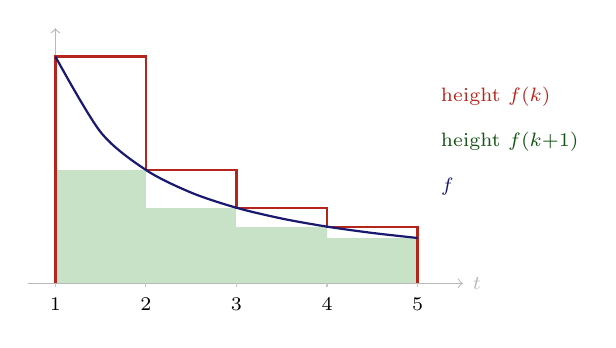
\begin{tikzpicture}[x=1.15cm,y=0.72cm]
  \draw[gray!55,->] (0.7,0) -- (5.5,0) node[right,font=\scriptsize] {$t$};
  \draw[gray!55,->] (1,0) -- (1,4.5);
  \foreach \k in {1,2,3,4,5} {
    \draw[gray!45] (\k,0.06) -- (\k,-0.06);
    \node[font=\scriptsize,anchor=north] at (\k,-0.08) {$\k$};
  }
  % right bars (lower): height f(k+1) on [k,k+1], drawn first
  \fill[ForestGreen!25] (1,0) rectangle (2,2);
  \fill[ForestGreen!25] (2,0) rectangle (3,1.333);
  \fill[ForestGreen!25] (3,0) rectangle (4,1);
  \fill[ForestGreen!25] (4,0) rectangle (5,0.8);
  % left bars (upper outline)
  \draw[BrickRed,line width=0.8pt] (1,0) -- (1,4) -- (2,4) -- (2,2) -- (3,2) -- (3,1.333) -- (4,1.333) -- (4,1) -- (5,1) -- (5,0.8) -- (5,0);
  \draw[MidnightBlue,thick] plot[smooth] coordinates {(1,4) (1.5,2.667) (2,2) (2.5,1.6) (3,1.333) (3.5,1.143) (4,1) (4.5,0.889) (5,0.8)};
  \node[font=\scriptsize,BrickRed,anchor=west] at (5.15,3.3) {height $f(k)$};
  \node[font=\scriptsize,ForestGreen!60!black,anchor=west] at (5.15,2.5) {height $f(k{+}1)$};
  \node[font=\scriptsize,MidnightBlue,anchor=west] at (5.15,1.7) {$f$};
\end{tikzpicture}
